\subsection{Iterative Architecture Evolution}

\subsubsection{Development Methodology}

A spiral development model was adopted, with each iteration addressing specific performance bottlenecks identified through empirical analysis. This approach enabled systematic optimization while maintaining system stability throughout the development process.

\subsection{Iteration 1: Baseline Sequential Processing}

\subsubsection{Implementation Approach:} Initial architecture processed translation requests sequentially, converting JSON objects to string arrays and submitting single requests to LibreTranslate.

\subsubsection{Performance Baseline:}
\begin{itemize}
    \item Average response time: 2.3 seconds for typical cultural tips requests
    \item Concurrent user limit: $\sim$10 users before significant performance degradation
    \item Translation accuracy: 98.5\% successful completion rate
\end{itemize}

\subsubsection{Bottleneck Analysis:} Sequential processing created obvious performance limitations, particularly with large cultural tips datasets containing multiple text segments of varying lengths.

\textbf{Key Learning:} The baseline established that single-threaded processing was insufficient for production requirements, validating the need for parallel processing architecture.

\begin{figure}[H]
    \centering
    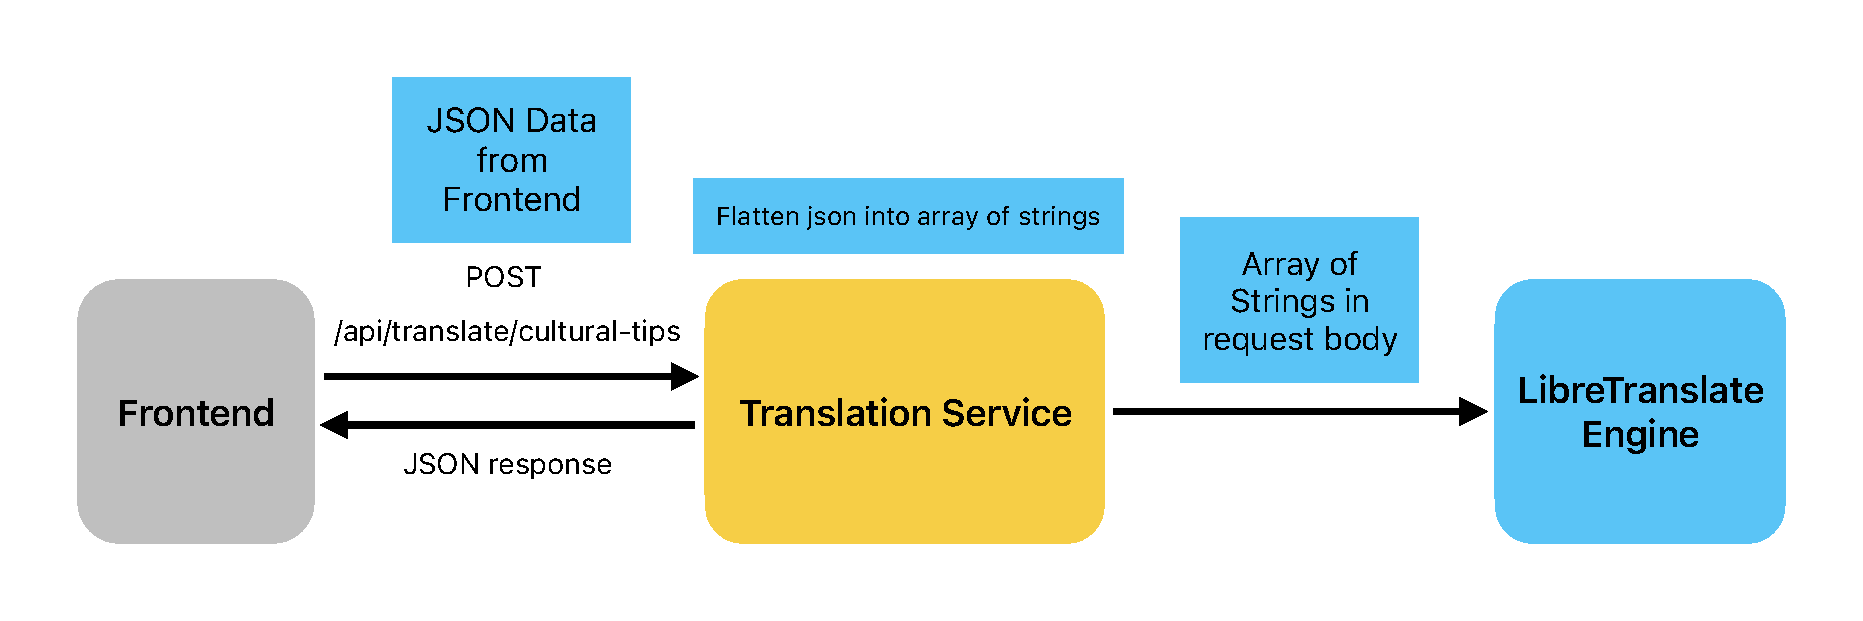
\includegraphics[width=1\linewidth]{chapter/05_implementation/backend/B_architectural_design/Backend_Initial_Concept.pdf}
    \caption{Initial iteration of backend service}
    \label{fig:backend_iteration_1}
\end{figure}

\subsection{Iteration 2: Parallel Processing Implementation}

\subsubsection{Hypothesis:} Concurrent translation requests would reduce response time proportionally to the number of parallel processes.

\subsubsection{Technical Implementation:}
\begin{itemize}
    \item OpenNLP sentence splitter integration for semantic text segmentation (93\% accuracy)
    \item Greedy algorithm for load distribution across 4 parallel translation batches
    \item Enhanced \texttt{SentenceContext} object with batch numbering and indexing
\end{itemize}

\subsubsection{Results Analysis:}
\begin{itemize}
    \item Response time improvement: 20\% reduction from baseline
    \item Unexpected finding: Minimal performance gain despite 4-way parallelization
    \item Resource utilization: Suboptimal due to uneven batch processing times
\end{itemize}

\subsubsection{Root Cause Investigation:} LibreTranslate's internal threading limitations prevented effective parallel processing within a single instance. The bottleneck shifted from request serialization to translation engine capacity, indicating the need for horizontal scaling rather than vertical optimization.

\textbf{Critical Insight:} Single-instance optimization has natural limits; distributed processing architecture required for significant performance improvements.

\begin{figure}[H]
    \centering
    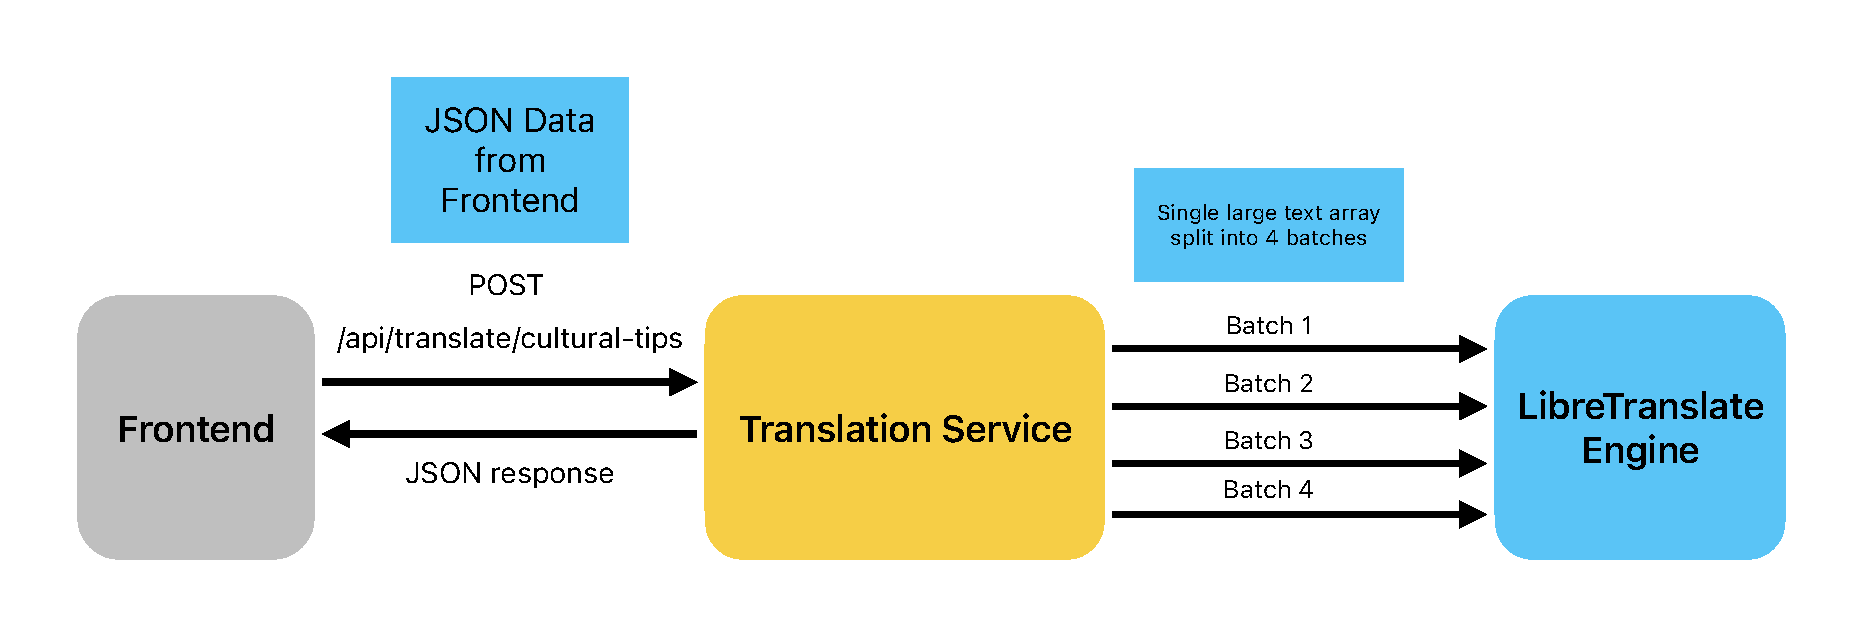
\includegraphics[width=1\linewidth]{chapter/05_implementation/backend/B_architectural_design/Backend_Iteration_2.pdf}
    \caption{Second iteration of backend service}
    \label{fig:backend_iteration_2}
\end{figure}

\subsection{Iteration 3: Horizontal Scaling with Service Discovery}

\subsubsection{Architectural Decision:} Transition from vertical optimization to horizontal scaling using multiple LibreTranslate instances.

\subsubsection{Technical Challenges:}
\begin{itemize}
    \item Kubernetes load balancing inefficiencies with REST client connection pooling
    \item Single connection pool routing requests to individual instances despite cluster configuration
    \item CPU-based auto-scaling triggering without effective load distribution
\end{itemize}

\subsubsection{Solution Architecture:}
Netflix Eureka service discovery implementation providing:
\begin{itemize}
    \item Intelligent load distribution across available translation engine instances
    \item Dynamic instance discovery and health monitoring
    \item Fine-grained control over request routing algorithms
\end{itemize}

\subsubsection{Wrapper Service Design:}
A dedicated wrapper service was implemented to bridge LibreTranslate (Docker container) with Eureka service discovery:
\begin{itemize}
    \item 1:1 coupling between wrapper service and LibreTranslate instance
    \item Automatic service registration and health checks
    \item Kubernetes-based auto-scaling triggered at 60\% CPU threshold
\end{itemize}

\subsubsection{Performance Results:}
\begin{itemize}
    \item Response time improvement: 60\% reduction from baseline architecture
    \item Scalability validation: Linear performance scaling with instance count
    \item Cost efficiency: Resource utilization optimized through dynamic scaling policies
\end{itemize}

\textbf{Critical Success Factor:} Service discovery patterns proved more effective than relying solely on Kubernetes native load balancing for this specific use case, providing greater control over request distribution strategies.

\begin{figure}[H]
    \centering
    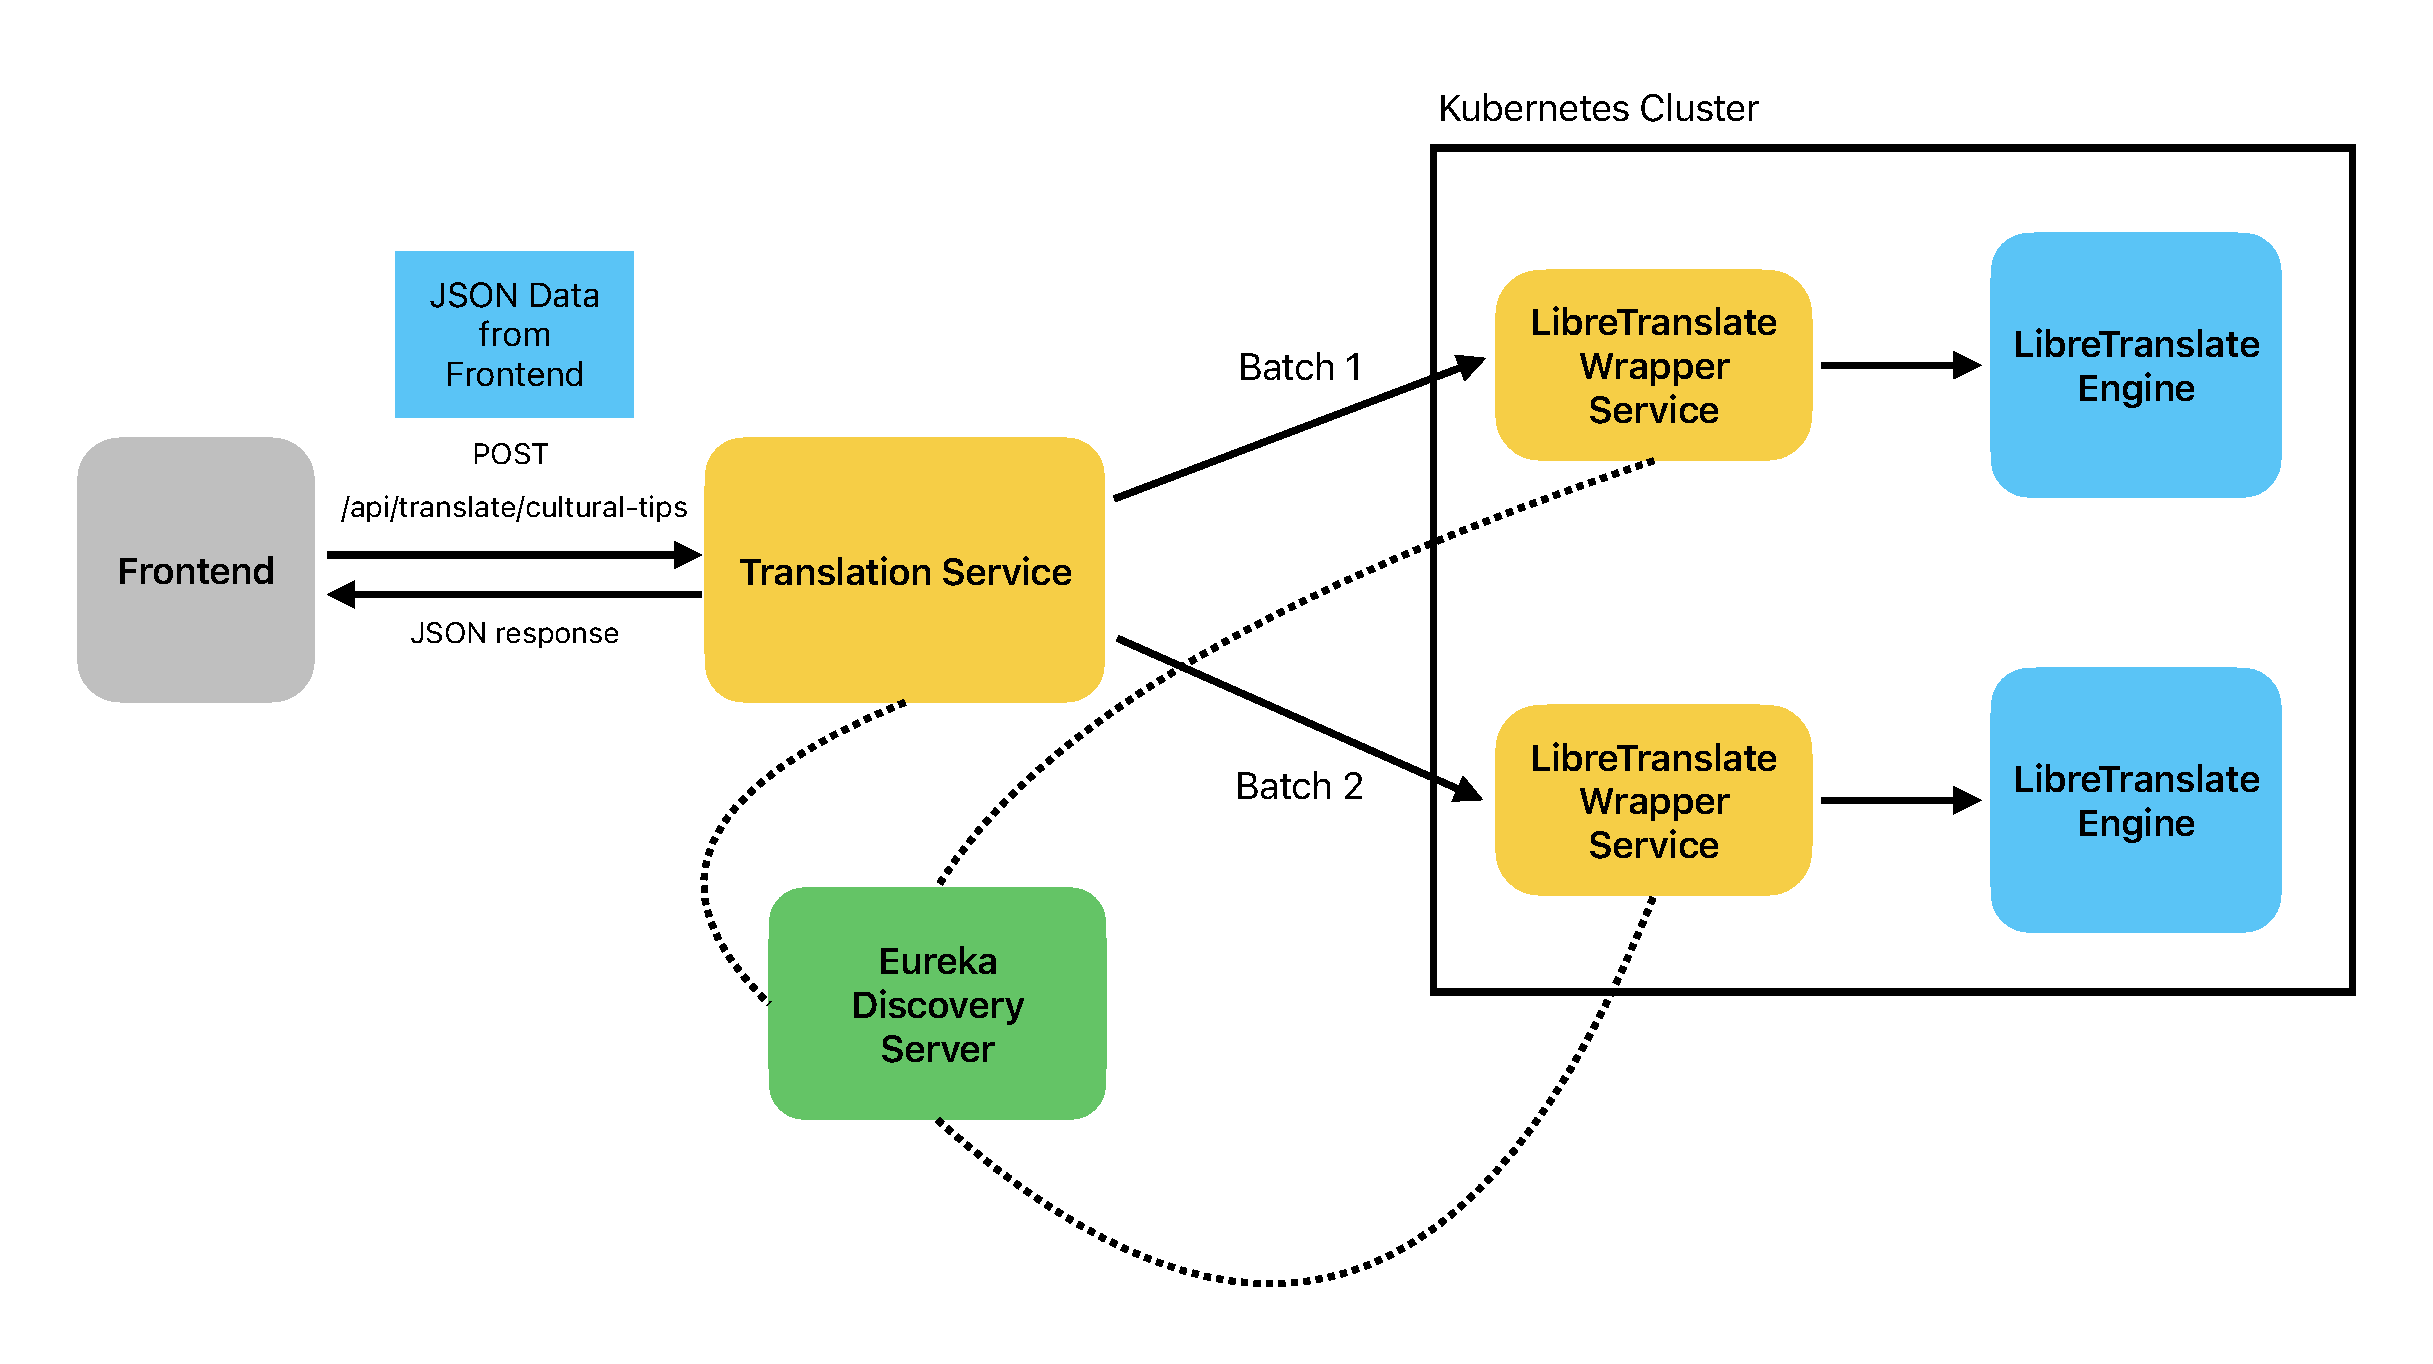
\includegraphics[width=1\linewidth]{chapter/05_implementation/backend/B_architectural_design/Backend_Iteration_3.pdf}
    \caption{Third iteration of backend service}
    \label{fig:backend_iteration_3}
\end{figure}

\subsection{Iteration 4: Caching Layer and Database Integration}

\subsubsection{Problem Identification:} Each frontend request triggered both AI agent calls for cultural tips generation and translation engine processing, resulting in:
\begin{itemize}
    \item High AI API costs per user session
    \item Redundant translation processing for identical city data
    \item Unnecessary computational overhead for static cultural content
\end{itemize}

\subsubsection{Solution Architecture:}
Implementation of a comprehensive caching strategy with database persistence:

\subsubsection{Database Schema Design:}
\begin{itemize}
    \item City data storage with 30-day refresh cycles
    \item Language-specific translation caching
    \item Request frequency tracking for cache optimization
\end{itemize}

\subsubsection{API Endpoint Enhancement:}
New endpoint \texttt{/api/v2/tips} with backward compatibility maintenance:

\subsubsection{Processing Logic:}
\begin{enumerate}
    \item Database query for existing city data in target language
    \item AI agent invocation only for cache misses
    \item English content storage for base translation processing
    \item Translated content caching for subsequent requests
    \item Direct database response for cache hits
\end{enumerate}

\subsubsection{Performance Impact:}
\begin{itemize}
    \item AI API cost reduction: 85\% decrease through cache hit optimization
    \item Translation processing reduction: 70\% improvement for repeated requests
    \item Overall response time: 40\% improvement for cached content requests
\end{itemize}

\begin{figure}[H]
    \centering
    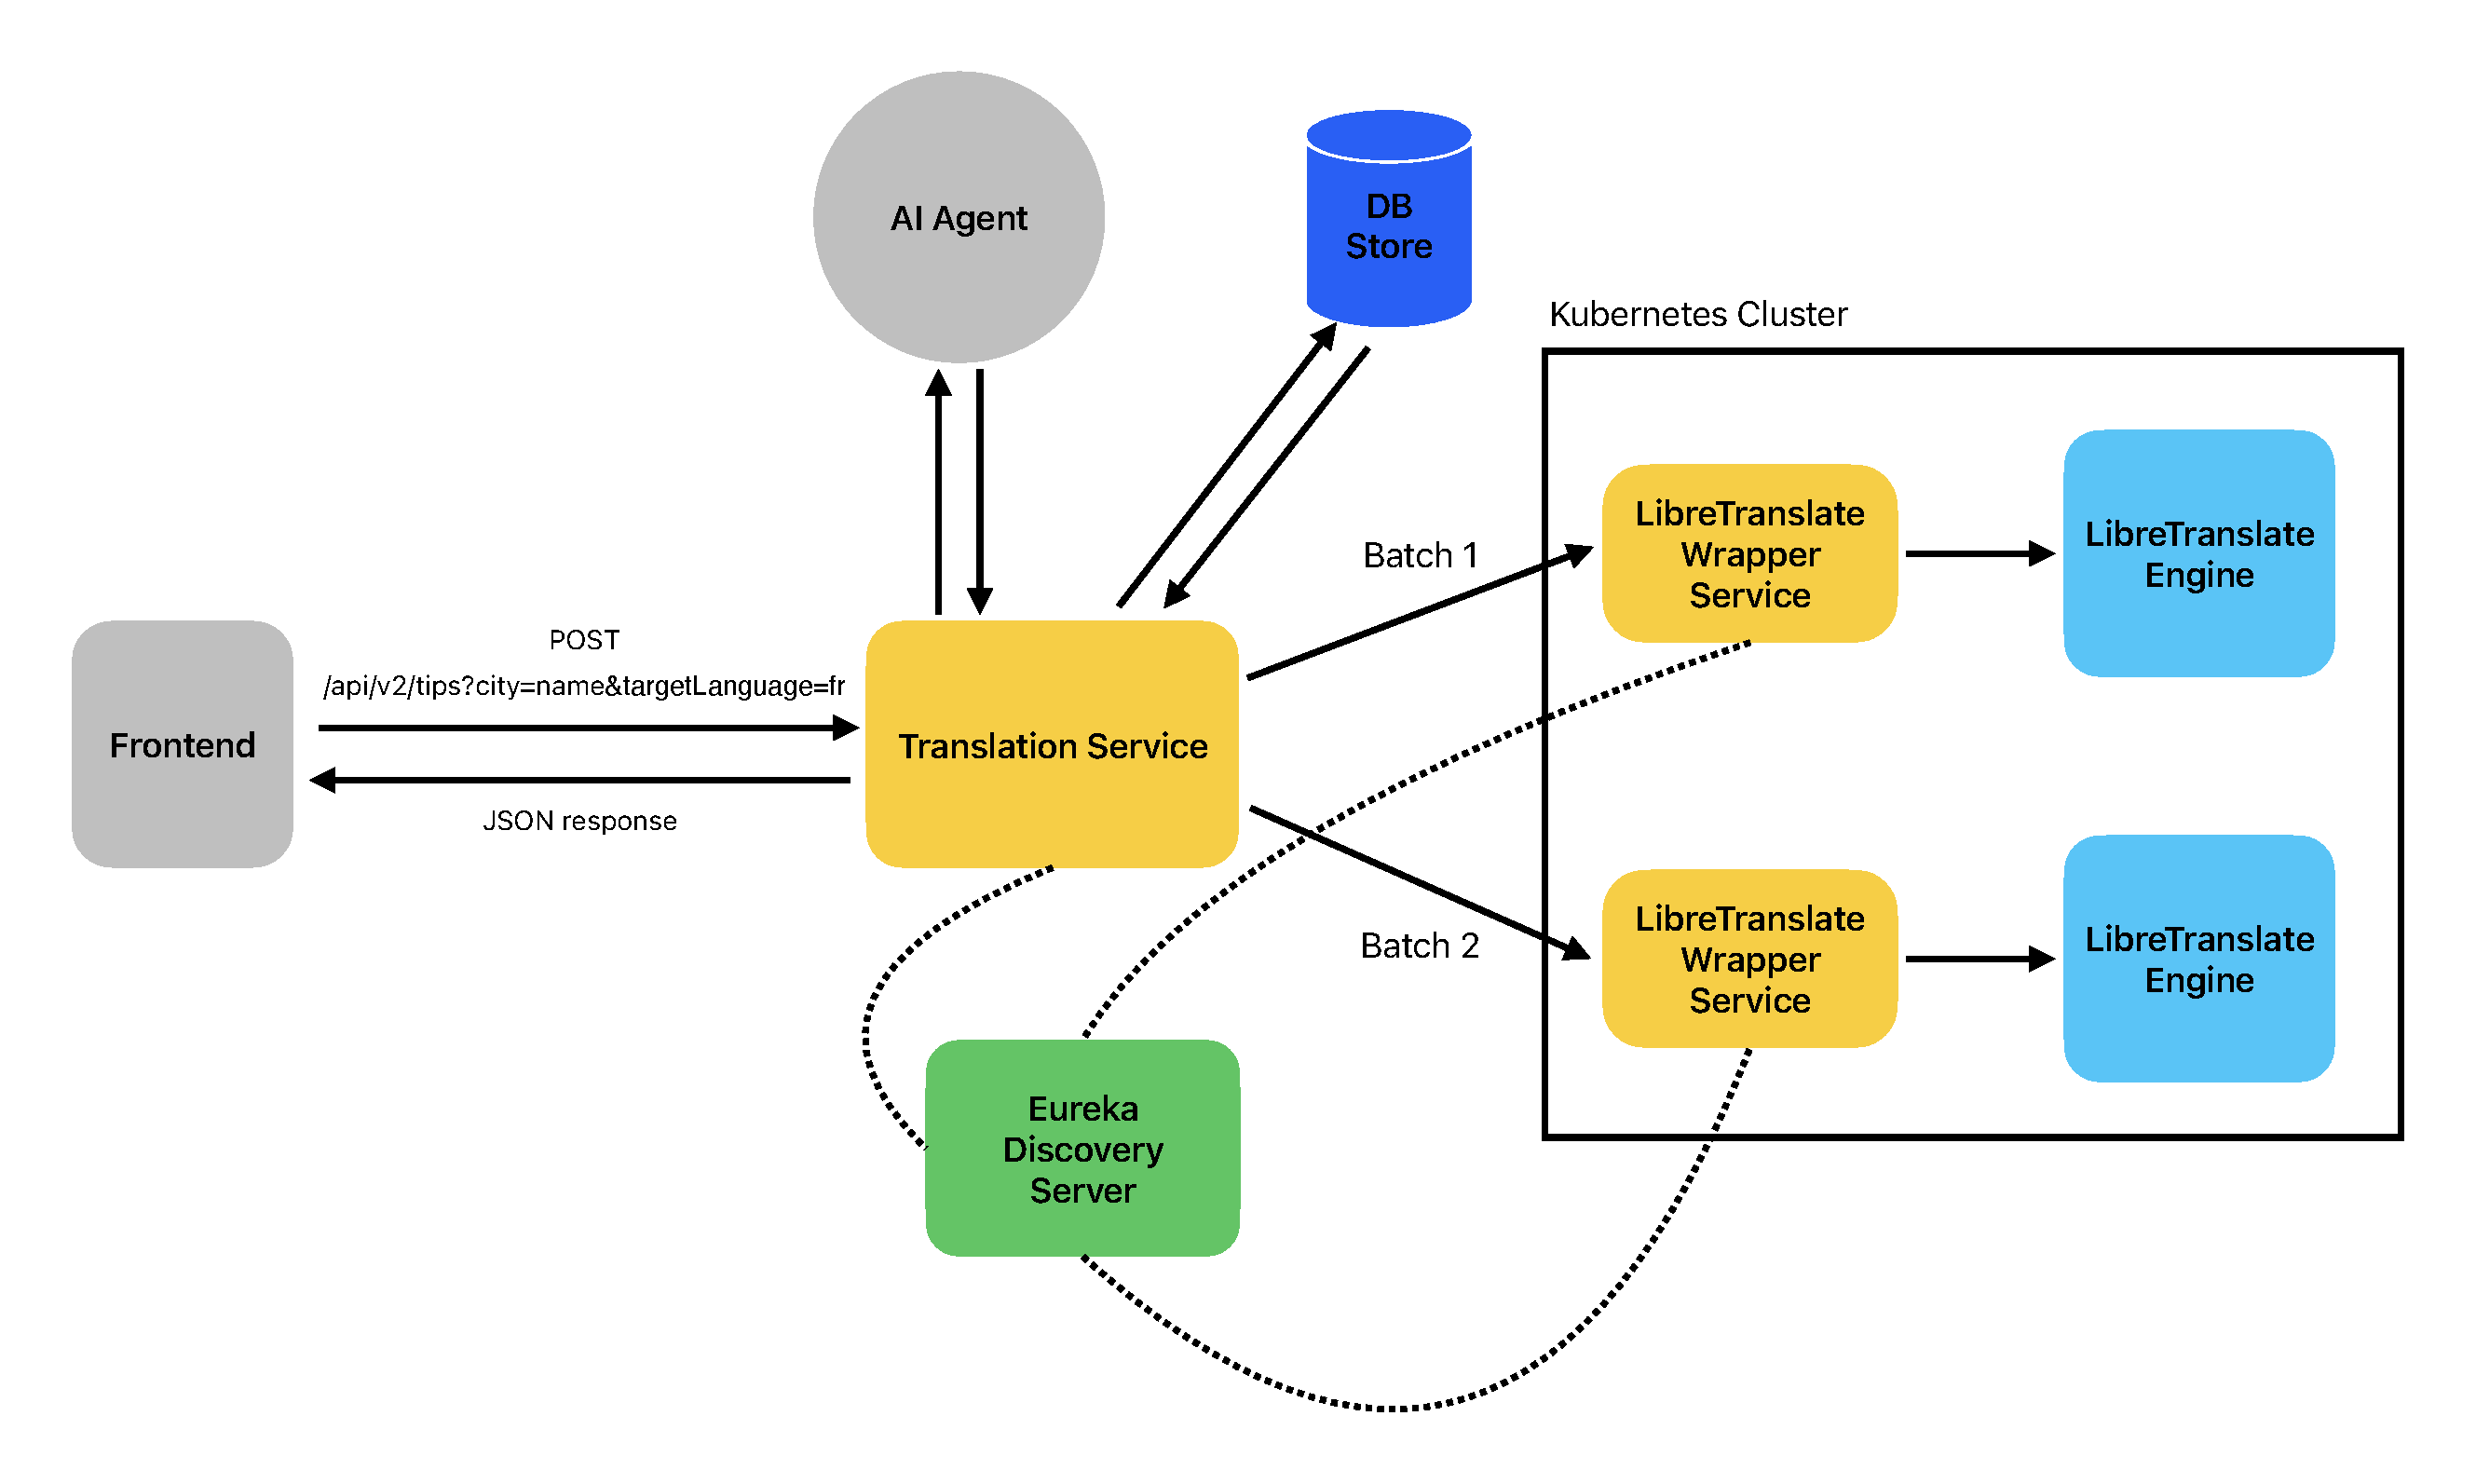
\includegraphics[width=1\linewidth]{chapter/05_implementation/backend/B_architectural_design/Backend_Iteration_4.pdf}
    \caption{Fourth iteration of backend service}
    \label{fig:backend_iteration_4}
\end{figure}

\begin{figure}[H]
    \centering
    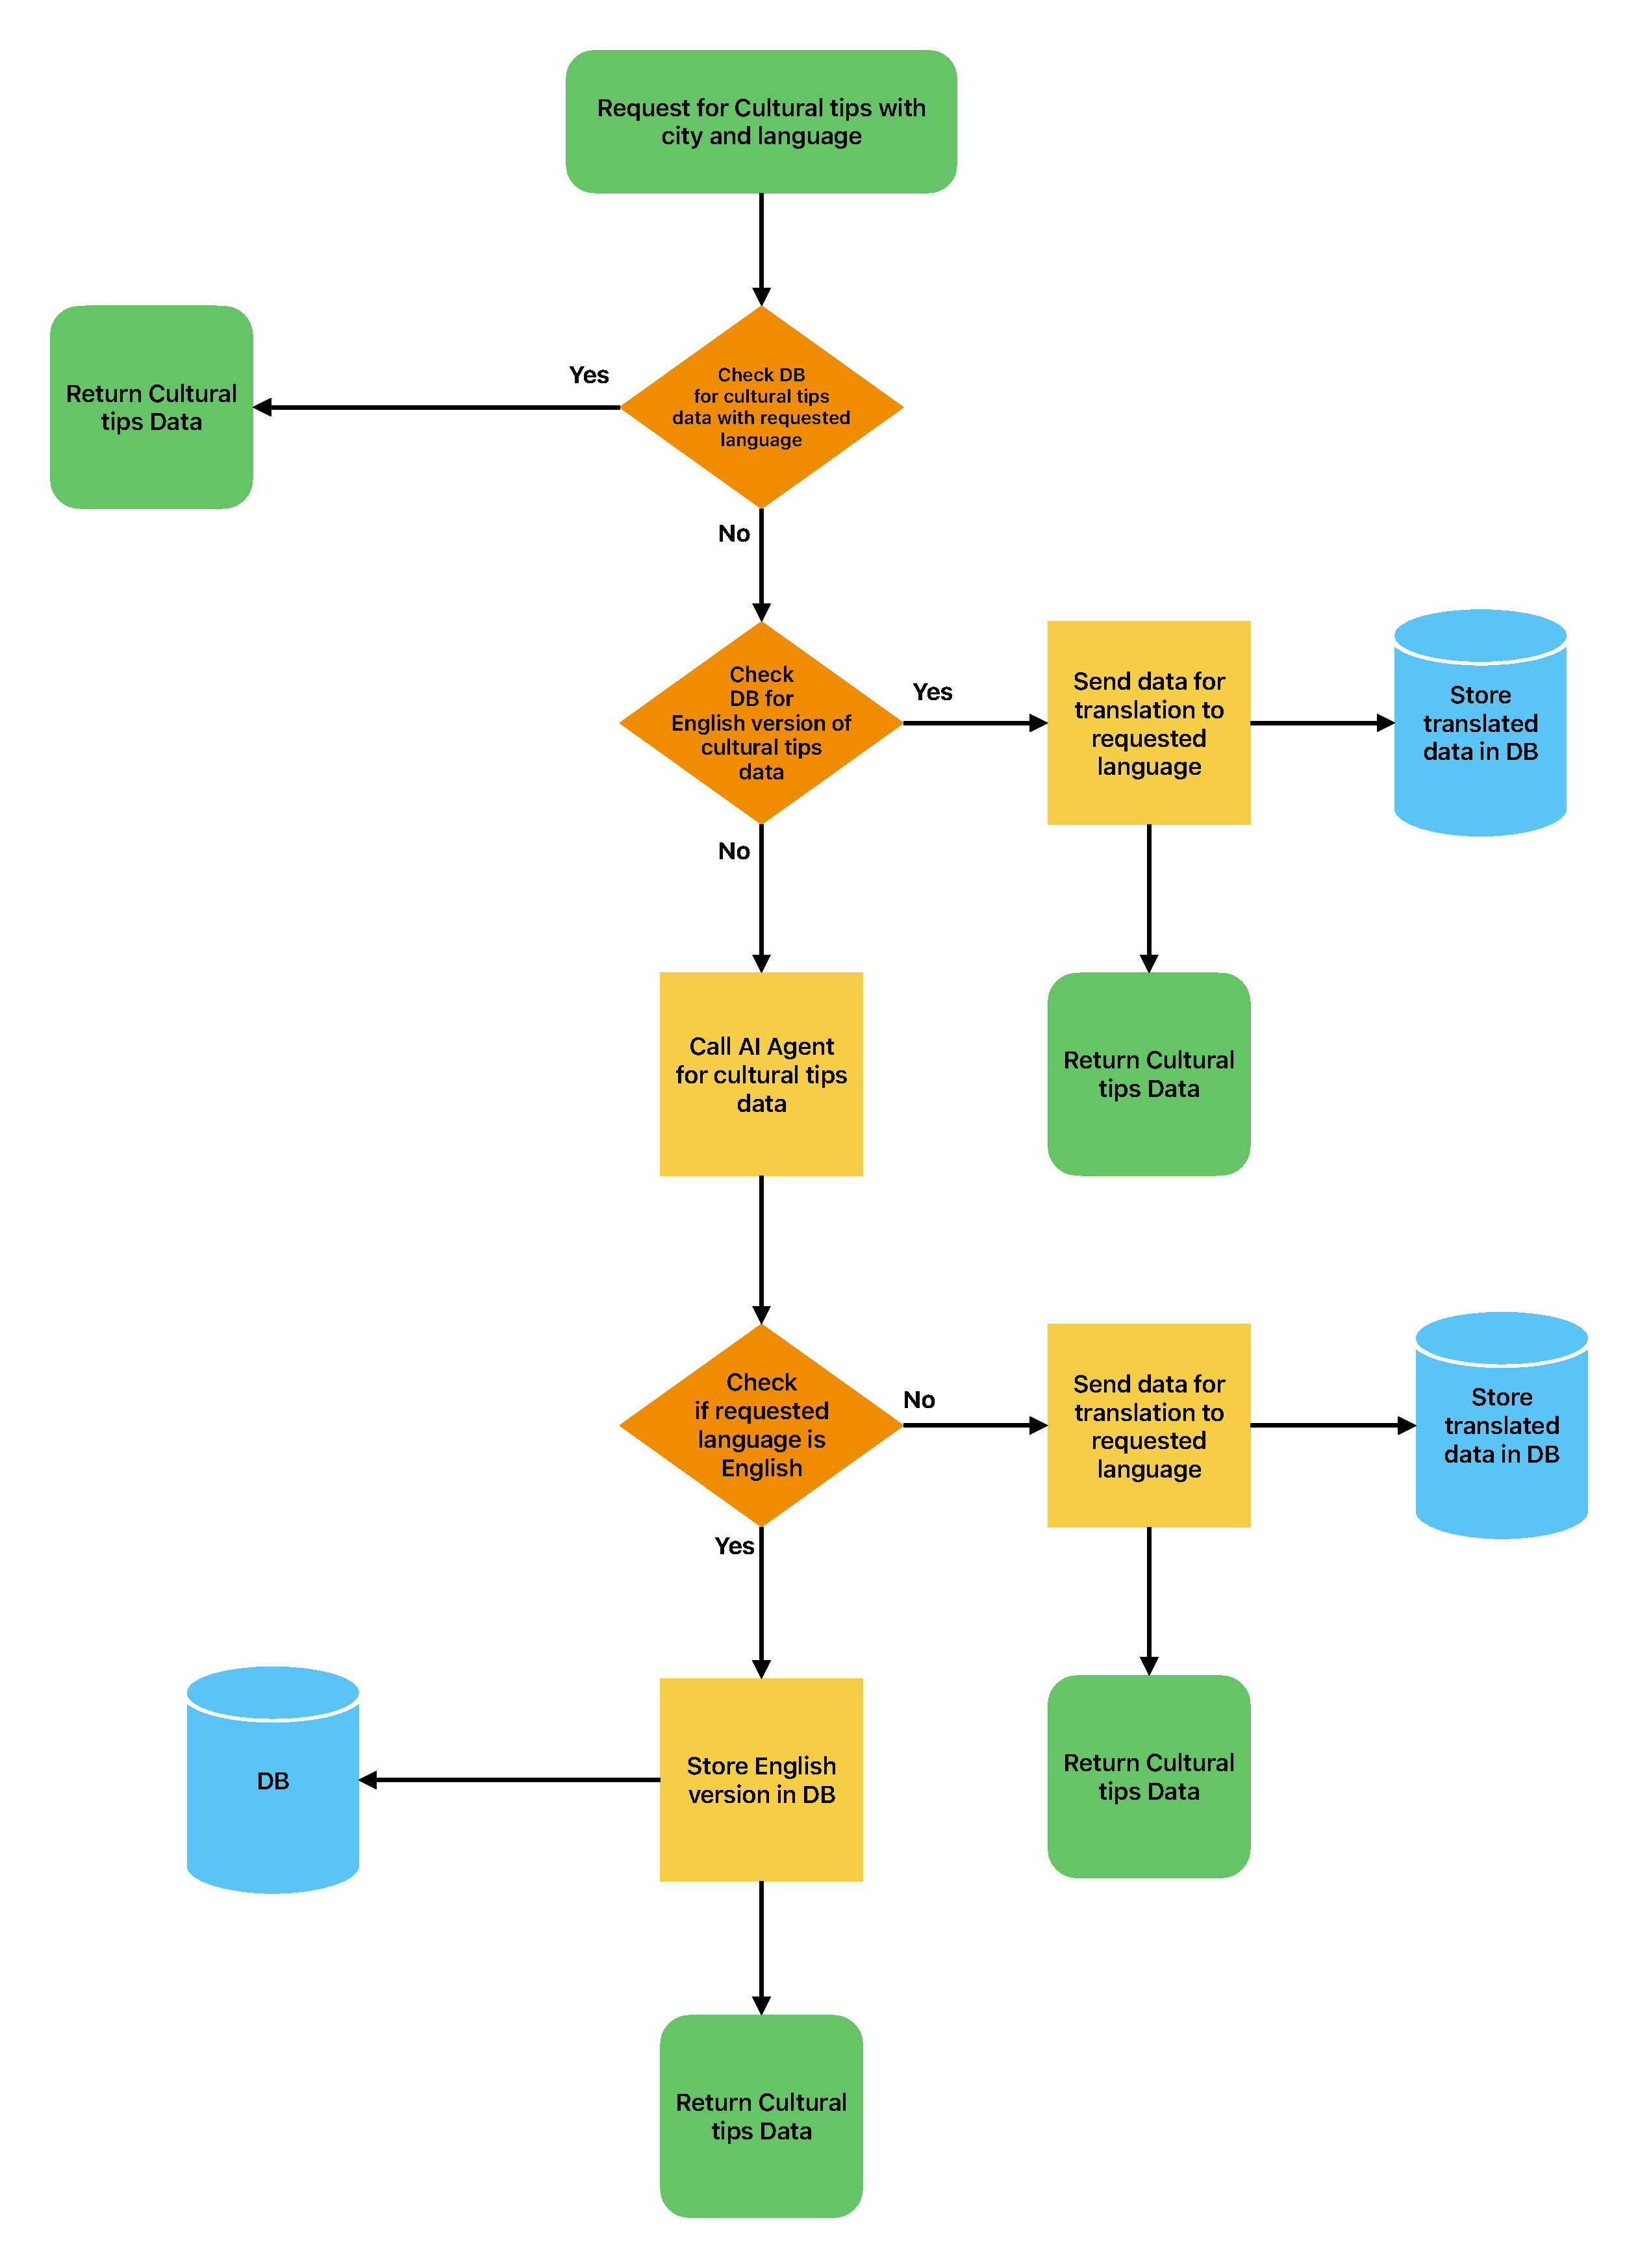
\includegraphics[width=1\linewidth]{chapter/05_implementation/backend/B_architectural_design/Business_Logic_Flow.pdf}
    \caption{Final business logic flow}
    \label{fig:backend_business_logic _flow}
\end{figure}